% Copyright 2019 Matheus Nunes <mhnnunes@dcc.ufmg.br>
% This program is free software: you can redistribute it and/or modify
% it under the terms of the GNU General Public License as published by
% the Free Software Foundation, either version 3 of the License, or
% (at your option) any later version.

% This program is distributed in the hope that it will be useful,
% but WITHOUT ANY WARRANTY; without even the implied warranty of
% MERCHANTABILITY or FITNESS FOR A PARTICULAR PURPOSE.  See the
% GNU General Public License for more details.

% You should have received a copy of the GNU General Public License
% along with this program.  If not, see <http://www.gnu.org/licenses/>.

\documentclass[sigconf]{acmart}

\usepackage{booktabs} % For formal tables
\usepackage[brazil]{babel}
%\usepackage[T1]{fontenc}
\usepackage[utf8]{inputenc}  
\usepackage{textcomp}

%\usepackage[numbers]{natbib} % for \citeauthor

\usepackage{subcaption}
\usepackage{footnote}
\usepackage{float}
\usepackage{hyperref} % colored links

\usepackage{color}				% Controle das cores

\usepackage[linesnumbered,lined,commentsnumbered]{algorithm2e}
\usepackage{algpseudocode}
\usepackage{program}
\SetAlgorithmName{Algoritmo}{algorithm}{Lista de algoritmos}

\newcommand{\matheus}[1]{ \textbf{\color{magenta}{Matheus: #1}} }
\newcommand{\tarsila}[1]{ \textbf{\color{blue}{Tarsila: #1}} }

 
\newtheorem{theorem}{\textbf{Teorema}}
\newtheorem{lemma}{\textbf{Lema}}

% Copyright
\setcopyright{none}

%Conference
\acmConference[PAA]{Trabalho Prático 1 - Grafos}{Maio 2019}{DCC-UFMG, Belo Horizonte, MG}
\acmYear{2019}
\copyrightyear{2019}


\begin{document}
\title{Trabalho Prático 1 - Grafos}
\subtitle{Projeto e Análise de Algoritmos, 2019-1}


\author{Matheus Henrique do Nascimento Nunes}
\affiliation{%
  \institution{Universidade Federal de Minas Gerais}
  \streetaddress{Av. Presidente Antônio Carlos, 6627}
  \city{Belo Horizonte}
  \state{Minas Gerais}
  \postcode{43017-6221}
}
\email{mhnnunes@dcc.ufmg.br}

% The default list of authors is too long for headers.
\renewcommand{\shortauthors}{Nunes, Matheus}


% REMOVE ACM REFERENCE FORMAT - MATHEUS
\settopmatter{printacmref=false}

\renewcommand\footnotetextcopyrightpermission[1]{} % removes footnote with conference information in first column


% ADD PAGE NUMBERING - MATHEUS
\settopmatter{printfolios=true}

\maketitle

\section{Introdução} \label{sec:introducao}

Batalhas intergaláticas são acontecimentos constantes em um futuro distante da humanidade. Frotas de naves espaciais são enviadas para combater forças inimigas em uma guerra cruel e infindável. O planejamento de um ataque surpresa a uma frota inimiga envolve duas atividades de suma importância: o reconhececimento de naves da frota inimiga e o cálculo do tempo de vantagem (tempo mínimo até todos os tripulantes das naves atingirem seu posto de trabalho correto e se prepararem para o ataque). Deseja-se que estas duas atividades sejam realizadas da melhor forma possível, logo o trabalho de alunos de Projeto e Análise de Algoritmos da UFMG foi requisitado.


\begin{figure*}[ht]
	\centering
	\begin{subfigure}[b]{0.24\textwidth}
		\centering
		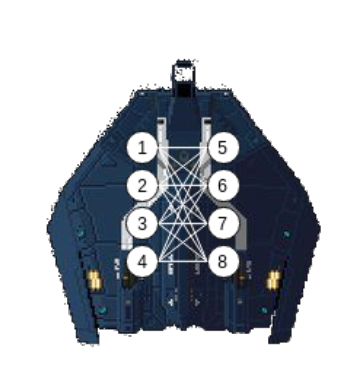
\includegraphics[width=0.9\textwidth]{imgs/bomb.png}
		\caption{Nave Bombardeira}
		\label{fig:nave_bomb}
	\end{subfigure}
	\begin{subfigure}[b]{0.24\textwidth}
		\centering
		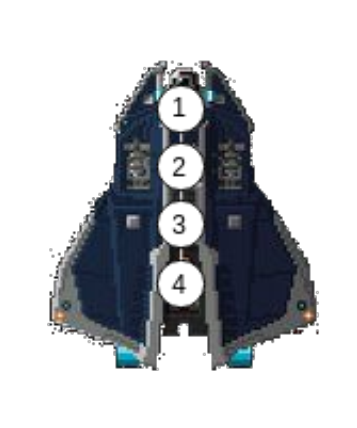
\includegraphics[width=0.9\textwidth]{imgs/rec.png}
		\caption{Nave de Reconhecimento}
		\label{fig:nave_rec}
	\end{subfigure}
	\begin{subfigure}[b]{0.24\textwidth}
		\centering
		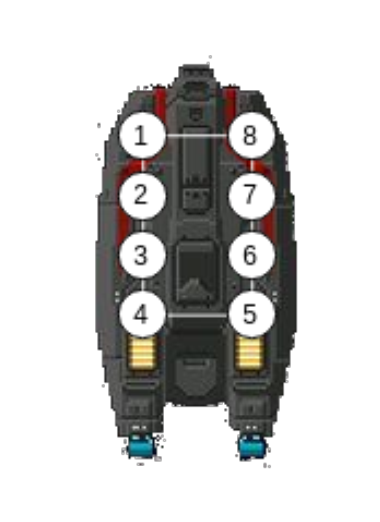
\includegraphics[width=0.9\textwidth]{imgs/trans.png}
		\caption{Nave de Transporte}
		\label{fig:nave_transp}
	\end{subfigure}
	\begin{subfigure}[b]{0.24\textwidth}
		\centering
		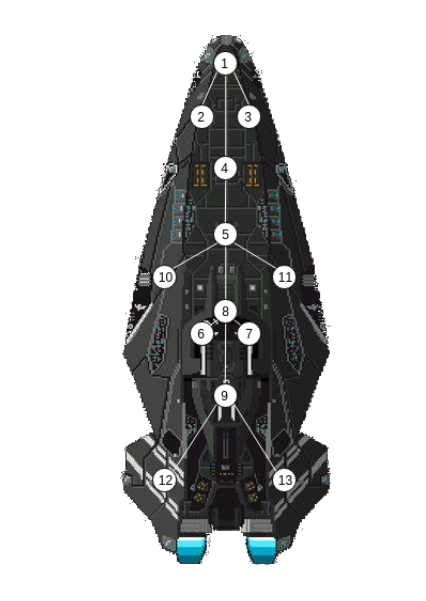
\includegraphics[width=0.9\textwidth]{imgs/frig.png}
		\caption{Nave Frigata}
		\label{fig:nave_frig}
	\end{subfigure}
	\caption{Tipos de Naves da Frota Inimiga}
	\label{fig:naves_tipos}
\end{figure*}


Sabe-se que as frotas inimigas são divididas em quatro tipos de naves, ilustrados na figura \ref{fig:naves_tipos}: \textit{Bombardeiros} (\ref{fig:nave_bomb}),  \textit{Reconhecimento} (\ref{fig:nave_rec}),  \textit{Transportadoras} (\ref{fig:nave_transp}) e \textit{Frigatas} (\ref{fig:nave_frig}). Algumas restrições são impostas a estas naves, por exemplo: em uma nave bombardeira, cada fileira de postos deve possuir no mínimo dois postos de combate; já nas naves de reconhecimento e transporte, o teleporte só é possível entre postos diretamente adjacentes.

Sabe-se também que estas naves são organizadas em postos de combates, de forma que cada tripulante pode ocupar apenas um posto por vez e, para se movimentar entre os postos, os tripulantes devem utilizar o sistema de teleporte nativo da nave. Este sistema de teleporte funciona trocando dois tripulantes por vez, entre postos de combate.

O objetivo do trabalho prático, portanto, é: dado um conjunto de pontos, representando as naves das frotas inimigas e os postos de combate presentes em cada uma delas, conexões entre estes pontos, representando as possibilidades de teleporte entre os postos, e um conjunto de pares $(p_i, p_j)$ representando teleportes a serem realizados entre dois pontos em uma mesma nave: 
\begin{itemize}
    \item Reconhecer e classificar o tipo de cada uma das naves presentes na frota inimiga
    \item Calcular o tempo de vantagem para a frota aliada (tempo mínimo para que todos os teleportes especificados pelos pares de pontos $(p_i, p_j)$ sejam realizados)
\end{itemize}



\input{formalizacao.tex
\input{metodologia.tex}
\section{Análise Experimental} \label{sec:experimentos}

O objetivo desta seção é apresentar dados que demonstram o desempenho  do código entregue como resultado do trabalho prático.  Os experimentos foram realizados em uma máquina com processador Intel\textsuperscript{\textregistered} Core\textsuperscript{\texttrademark} i5-6200U, de 8 núcleos a $2.30GHz$. A máquina opera a $64$ bits, e possui $8$GB de memória RAM DIMM DDR4. O sistema operacional utilizado foi o Linux Mint Sonya $18.2$. O trabalho foi implementado na linguagem \texttt{C++11}. 

As instâncias de teste foram geradas utilizando um gerador de grafos aleatórios disponível online\footnote{\url{https://github.com/cgpimenta/util}}, utilizando 10 \textit{seeds} diferentes\footnote{$\{ 1, 6, 16, 18, 33, 57, 68, 75, 80, 99 \}$} para o gerador de numeros pseudo-aleatórios. Cinco grafos de cada tipo e uma versão completa com todos os tipos de grafo foram geradas, de cinco tamanhos diferentes de nós\footnote{$\{ 10, 20, 100, 1000, 10000, 100000 \}$} e arestas\footnote{$\{ 100, 1000, 10000, 100000, 1000000 \}$}. Utilizando todas as combinações destes parâmetros, o número total de instâncias geradas foi $320$.


\begin{figure}[h]
\centering
\includegraphics[width=1\linewidth]{../timeplot}
\caption{Gráfico de tempo de execução por número de nós}
\label{fig:timeplot}
\end{figure}


A figura \ref{fig:timeplot} apresenta os resultados do tempo de execução para as instâncias de teste. O eixo $x$ representa o número de nós da instância e o eixo $y$ representa o tempo de execução do programa. O tamanho do ponto representa o número de arestas da instância. Uma regressão LOESS (\textit{Locally Estimated Scatterplot Smoothing})\footnote{\url{https://blogs.sas.com/content/iml/2016/10/17/what-is-loess-regression.html}} foi ajustada aos pontos, a fim de revelar alguma tendência presente na relação. Pode-se observar que há um crescimento acelerado do tempo de processamento quando o numero de nós está entre 25 e 50 mil, porém este crescimento é causado pelo aumento no número de arestas (pode-se observar pelo tamanho do ponto que o número de arestas está próximo de 10 milhões). O comportamento da curva é aproximadamente quadrático em alguns pontos, mas sub-quadrático em outros, como esperado após a análise de complexidade teórica.


\begin{figure}[h]
\centering
\includegraphics[width=\linewidth]{../memoryplot}
\caption{Gráfico da memória utilizada por número de nós e arestas}
\label{fig:memoryplot}
\end{figure}

O gráfico da figura \ref{fig:memoryplot} apresenta os resultados para a memória utilizada pelo programa durante a execução. Pode-se observar que a curva gerada pela regressão é bem parecida com a da figura \ref{fig:timeplot}, assim como esperado após a análise teórica realizada na seção \ref{sec:metodologia}. O resultado  observado na prática é bem similar ao resultado teórico: para grafos densos ($\textbar E \textbar \approx \textbar V \textbar^2$, ou seja, muito mais arestas do que vértices) o comportamento do algoritmo será aproximadamente quadrático no número de nós.

Conclui-se que o objetivo do trabalho prático foi cumprido: implementar e analisar algoritmos em grafos. A resolução do problema passou por algoritmos exatos e algoritmos aproximativos, e a análise de complexidade teórica foi comprovada empiricamente.

\bibliographystyle{ACM-Reference-Format}
\bibliography{references.bib}

\end{document}
